\documentclass[answers]{exam}
\usepackage[english,spanish]{babel}
\usepackage[autostyle]{csquotes}
\usepackage[letterpaper,top=2cm,bottom=2cm,left=3cm,right=3cm,marginparwidth=1.75cm]{geometry}
\usepackage{amsmath, amssymb}
\usepackage{graphicx}
\usepackage{enumitem}
\usepackage{tikz,pgfplots}
\pgfplotsset{compat=1.18}
\usepackage[colorlinks=true, allcolors=blue]{hyperref}

\renewcommand{\solutiontitle}{\noindent\textbf{Respuesta:}\par\noindent}

% Header and footer
\pagestyle{headandfoot}
\firstpageheader{Universidad de Bolívar}{}{\selectlanguage{spanish}\today} 
\runningheader{Universidad de Bolívar}{}{Cálculo I}
\firstpagefooter{}{}{}
\runningfooter{}{\thepage}{}
\begin{document}

\begin{center}
	\Large\textbf{Cálculo I}\\[1em]
	\large\textbf{Corrección del Examen}\\[1em]
	\large Primer Ciclo \enquote*{A} - Ingeniería de Software\\[1em]
	% \large \today
\end{center}

\vspace{0.5cm}
\large\textbf{Estudiante}: Ariel Alejandro Calderón
\vspace{0.5cm}

\begin{questions}

	% Question 1
	\question \large\textbf{Para la función $\displaystyle y = \frac{x^3}{x^2 - 3} $ determine:}
	\begin{enumerate}[label=\alph*.]
		\item El dominio y recorrido.
		\item Si la función es par o impar.
		\item Estudie la monotonía.
	\end{enumerate}
	\begin{solution}
		\begin{enumerate}[label=\alph*.]
			\item El dominio de la función son todos los números reales excepto los valores que hacen el denominador igual a cero, es decir, $x^2 - 3 = 0 \Rightarrow x = \pm\sqrt{3}$. Por lo tanto, el dominio es $D = \mathbb{R} \setminus \{\pm\sqrt{3}\}$.

			\item La función no es ni par ni impar. Para comprobar esto, evaluamos $f(-x)$:
			      \[
				      f(-x) = \frac{(-x)^3}{(-x)^2 - 3} = \frac{-x^3}{x^2 - 3} \neq f(x) \text{ y } \neq -f(x)
			      \]

			\item La monotonía de la función se determina asi:
			      \begin{itemize}
				      \item \normalsize\textbf{Crece:} $\displaystyle
					            \left]-\infty, 3\right]\cup \left[3, \infty\right[
				            $
				      \item \normalsize\textbf{Decrece:} $\displaystyle
					            \left[-3, -\sqrt{3}\right[\cup \left]-\sqrt{3}, \sqrt{3}\right[\cup \left]\sqrt{3}, 3\right]
				            $
			      \end{itemize}
		\end{enumerate}
		\vspace{0.5cm}


		\begin{minipage}{\textwidth}
			\centering
			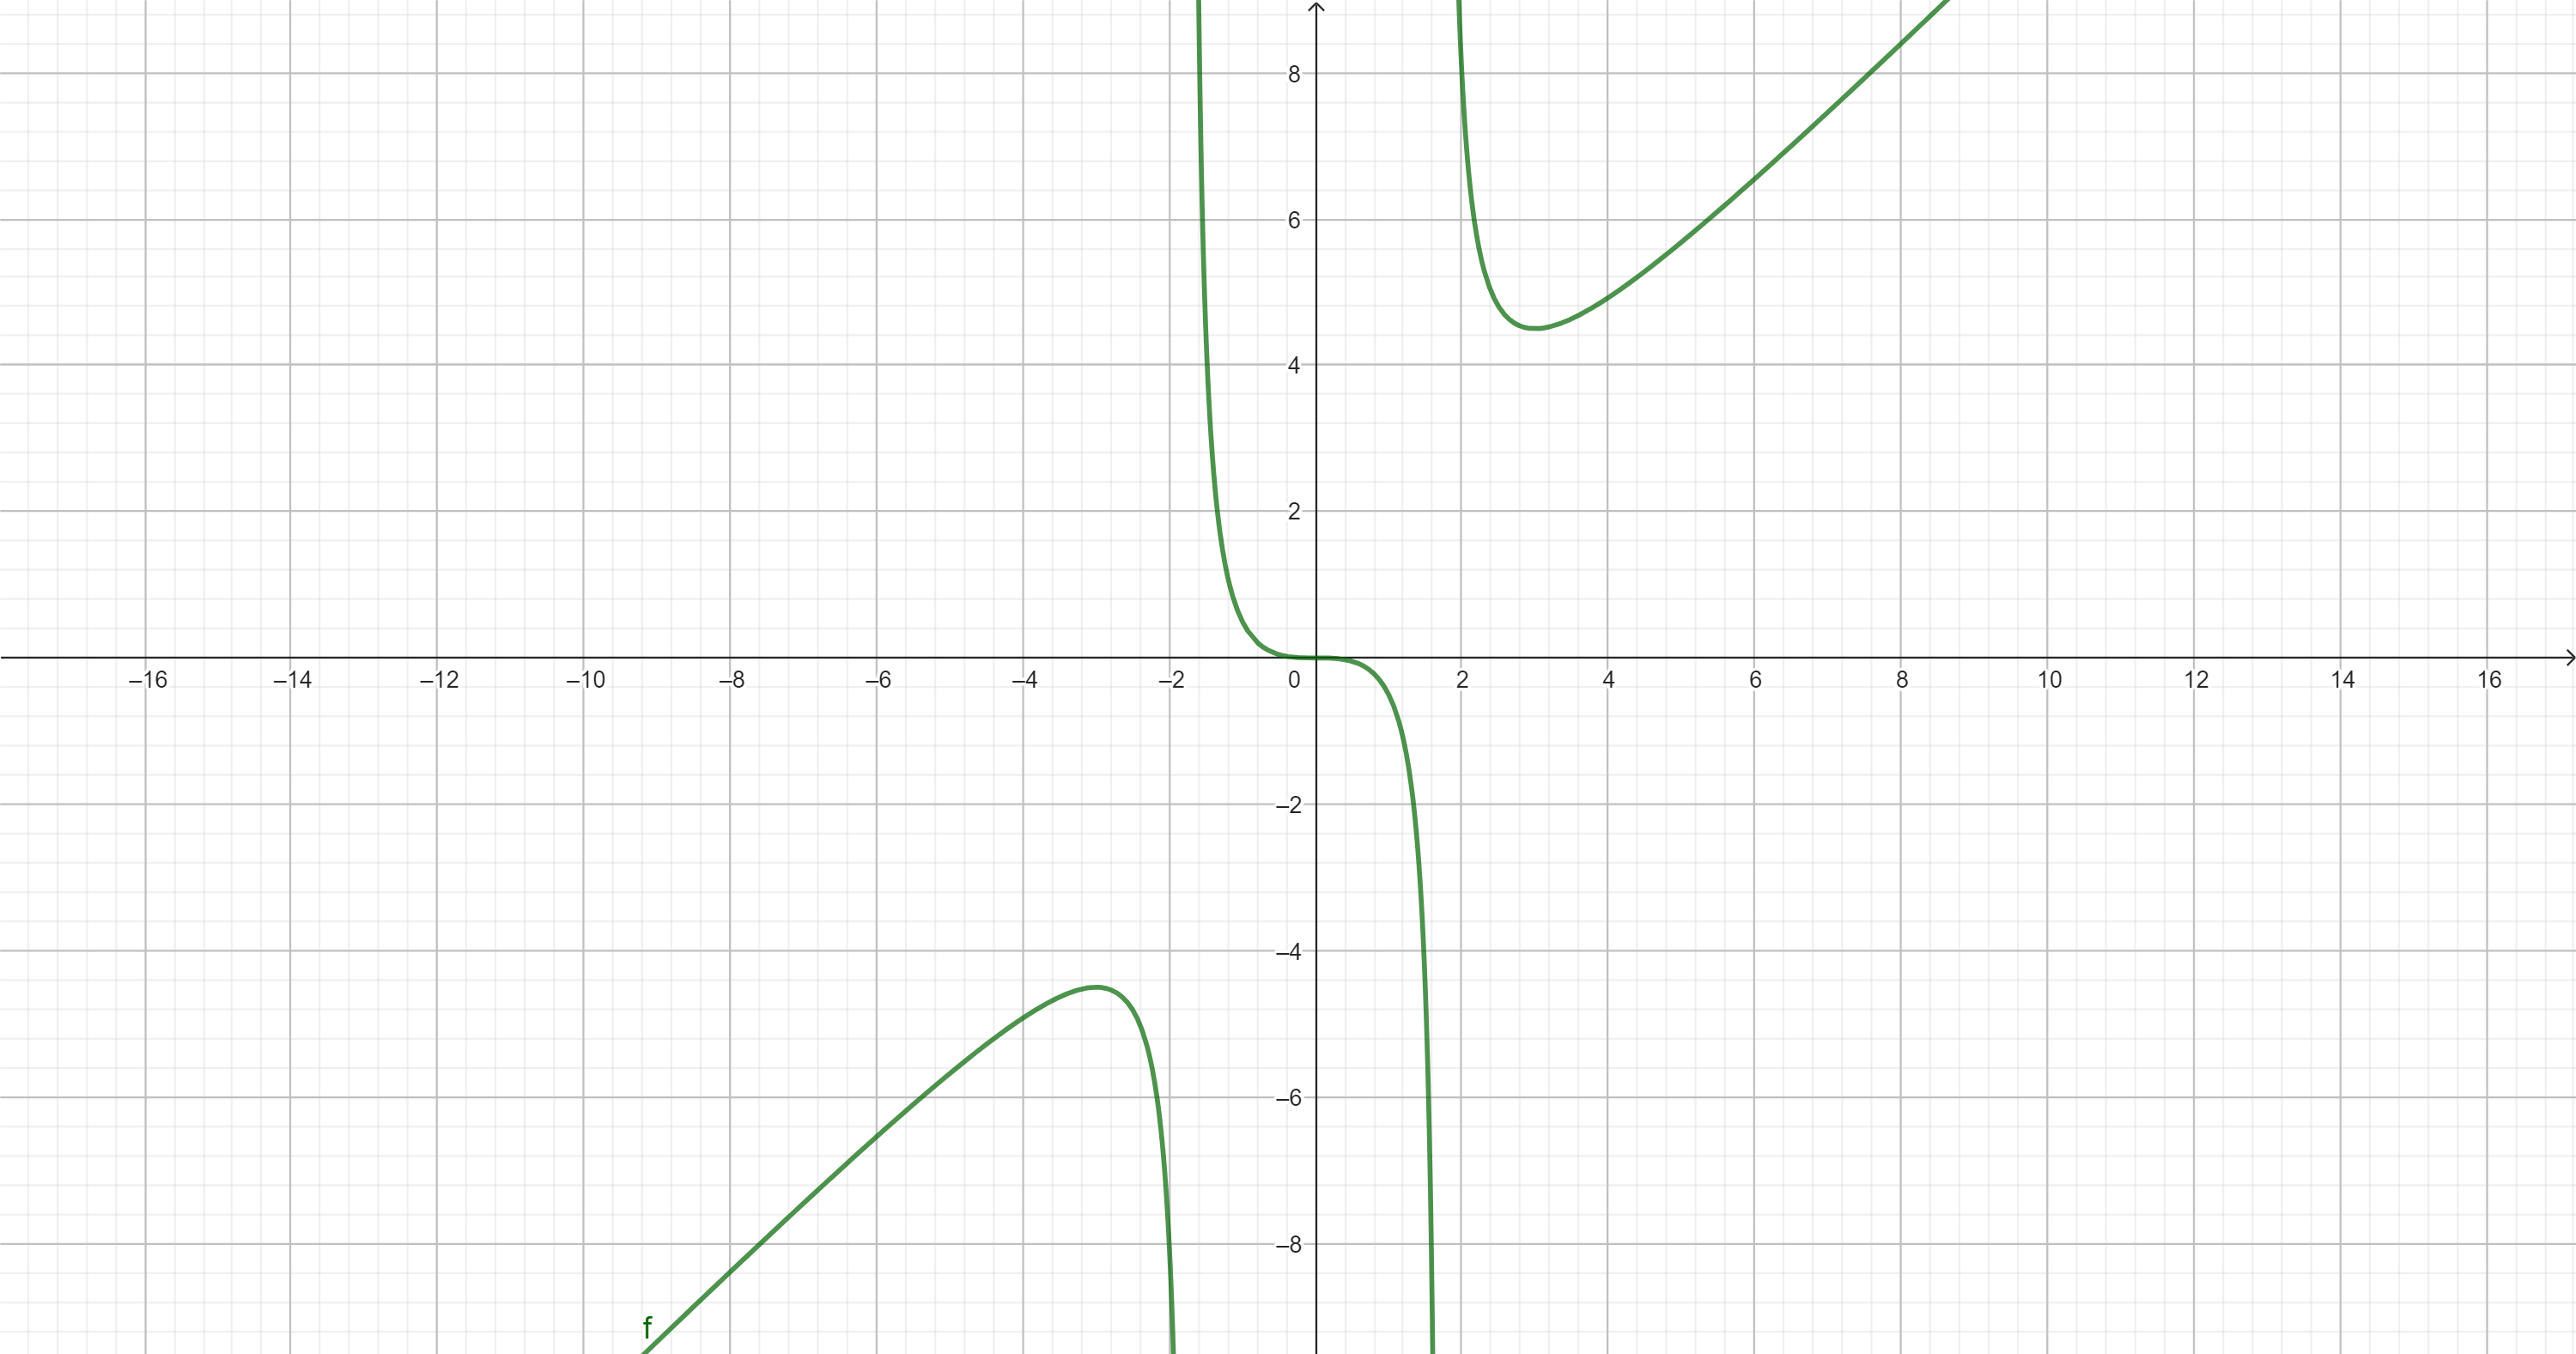
\includegraphics[width=0.9\textwidth]{public/g1.png}\\
		\end{minipage}
		\vspace{0.5cm}
	\end{solution}

	\vspace{0.5cm}

	% Question 2
	\question \large\textbf{Para la función $y = 1 + \tan x$ definida únicamente en el intervalo $\displaystyle \left]-\frac{\pi}{2}, \frac{\pi}{2}\right[$ determinar:}
	\begin{enumerate}[label=\alph*.]
		\item Si la función es biyectiva. Justifique su respuesta.
		\item Encuentre su inversa.
		\item Grafique en el mismo plano de la directa.
	\end{enumerate}
	\begin{solution}
		\begin{enumerate}[label=\alph*.]
			\item La función $y = 1 + \tan x$ es biyectiva en el intervalo dado porque es continua y estrictamente creciente en $\left]-\frac{\pi}{2}, \frac{\pi}{2}\right[$.

			\item Para encontrar la inversa, resolvemos $y = 1 + \tan x$ para $x$:
			      \[
				      y - 1 = \tan x \Rightarrow x = \tan^{-1}(y - 1)
			      \]
			      La inversa es $f^{-1}(y) = \tan^{-1}(y - 1)$.

			\item La gráfica de $y = 1 + \tan x$ y su inversa $y = \tan^{-1}(x - 1)$ se puede representar en el mismo plano.
		\end{enumerate}
		\vspace{0.5cm}
		\begin{minipage}{\textwidth}
			\centering
			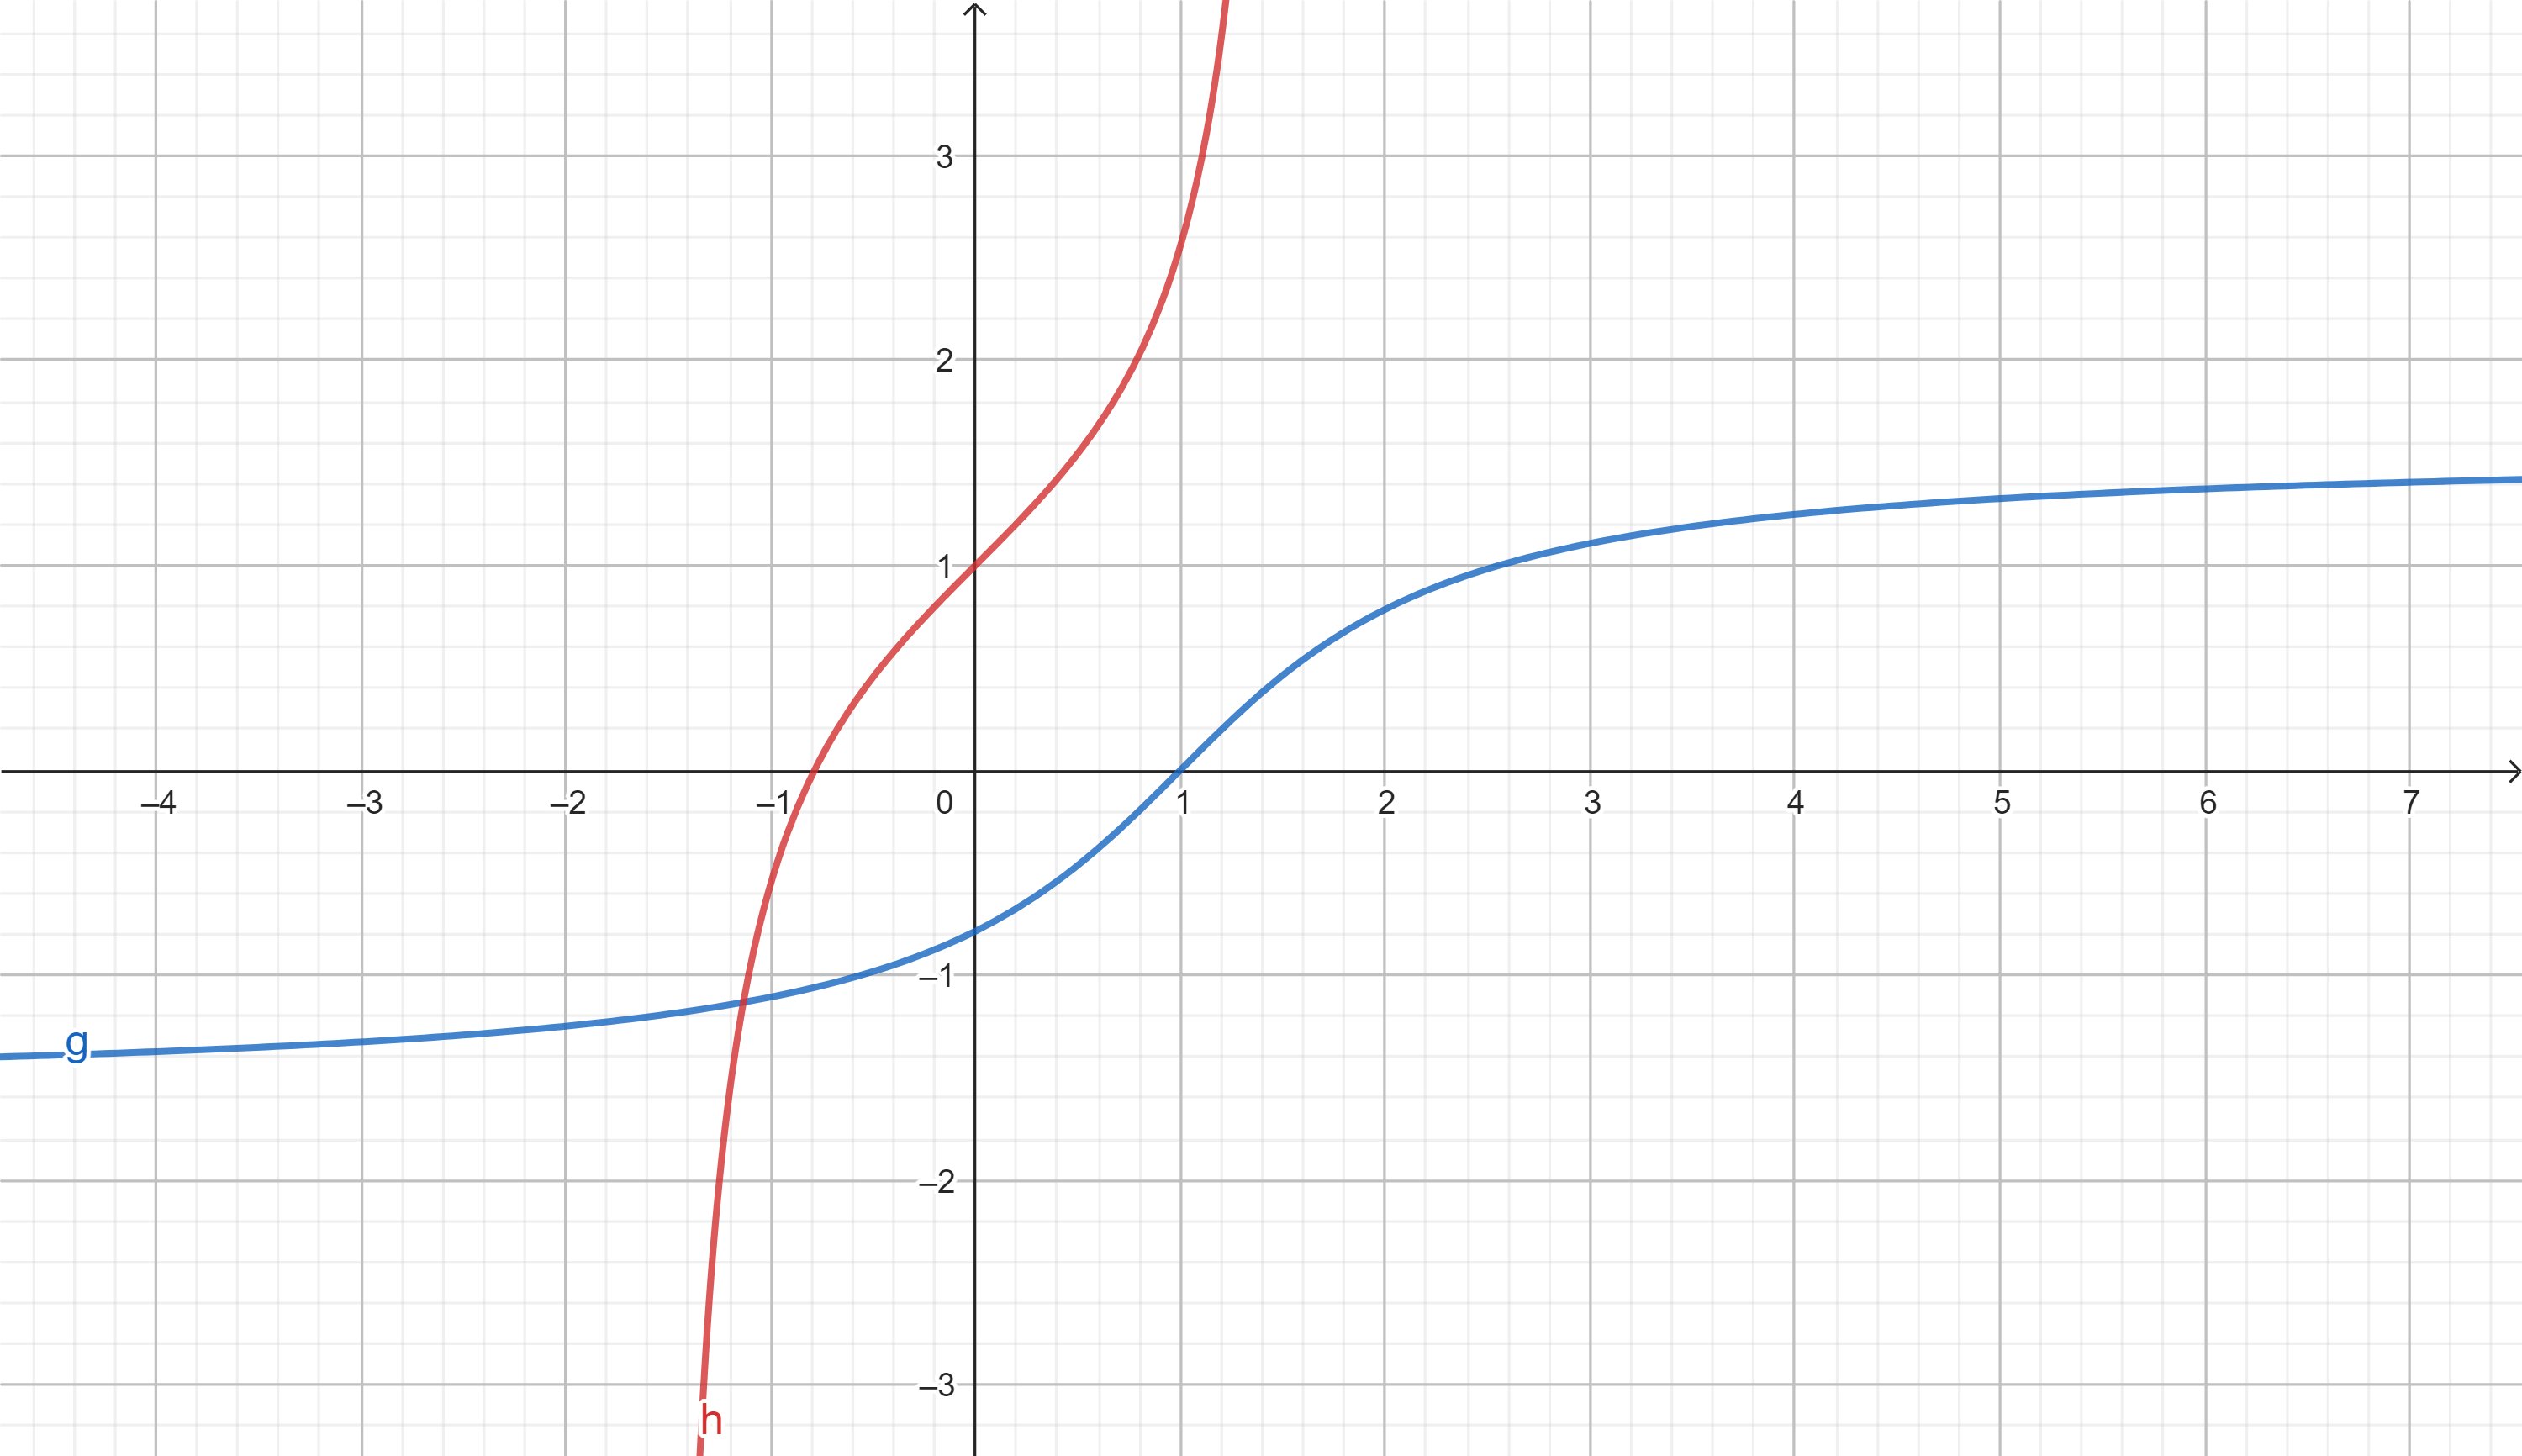
\includegraphics[width=0.9\textwidth]{public/g2.png}\\
		\end{minipage}
		\vspace{0.5cm}
	\end{solution}

	\newpage

	% Question 3
	\question \large\textbf{Para la función $\displaystyle f(x) = 3^{x-3}-2$ determine:}
	\begin{enumerate}[label=\alph*.]
		\item Su inversa si existe.
		\item Encuentre la función compuesta $f(f^{-1}(x))$.
	\end{enumerate}
	\begin{solution}
		\begin{enumerate}[label=\alph*.]
			\item Para encontrar la inversa, resolvemos $y = 3^{x-3} - 2$ para $x$:
			      \[
				      y + 2 = 3^{x-3} \Rightarrow x - 3 = \log_3(y + 2) \Rightarrow x = \log_3(y + 2) + 3
			      \]
			      La inversa es $f^{-1}(x) = \log_3(x + 2) + 3$.

			\item La función compuesta $f(f^{-1}(x))$ es:
			      \[
				      f(f^{-1}(x)) = f(\log_3(x + 2) + 3) = 3^{(\log_3(x + 2) + 3) - 3} - 2 = x + 2 - 2
			      \]
			      \[
				      f(f^{-1}(x)) = x
			      \]
		\end{enumerate}
		\vspace{0.5cm}
	\end{solution}

	\vspace{0.5cm}

	% Question 4
	\question \large\textbf{Calcular los límites indicados a continuación:}
	\begin{enumerate}[label=\alph*.]
		\item $\displaystyle \lim_{x\to{2}} \frac{\sqrt{3^x+7}}{x+2}$
		\item $\displaystyle \lim_{x\to{2}} \frac{x^3-4x}{x^2-3x+2}$
	\end{enumerate}
	\vspace{0.5cm}
	\begin{solution}
		\begin{enumerate}[label=\alph*.]
			\item Para el límite $\displaystyle \lim_{x\to{2}} \frac{\sqrt{3^x+7}}{x+2}$:
			      \[
				      \lim_{x \to 2} \frac{\sqrt{3^x+7}}{x+2} = \frac{\sqrt{3^2+7}}{2+2} = \frac{\sqrt{9+7}}{4} = \frac{\sqrt{16}}{4} = \frac{4}{4} = 1
			      \]

			\item Para el límite $\displaystyle \lim_{x\to{2}} \frac{x^3-4x}{x^2-3x+2}$:
			      \[
				      \lim_{x \to 2} \frac{x^3-4x}{x^2-3x+2} = \lim_{x \to 2} \frac{x(x^2-4)}{(x-1)(x-2)}= \frac{\infty}{\infty}
			      \]
			      Levantamos la indeterminación:
			      \[
				      x^3-4x = x(x^2-4) = x(x-2)(x+2)
			      \]
			      \[
				      \lim_{x \to 2} \frac{x(x-2)(x+2)}{(x-1)(x-2)} = \lim_{x \to 2} \frac{x(x+2)}{x-1}
			      \]
			      \vspace{0.1cm}
			      \[
				      = \frac{2(2+2)}{2-1} = \frac{2 \cdot 4}{1} = 8
			      \]
		\end{enumerate}
	\end{solution}

	\vspace{0.5cm}

	% End of questions
\end{questions}

\end{document}
